\documentclass{homework}
\course{Math 5522H}
\author{Jim Fowler}
\usepackage{amsmath}
\DeclareMathOperator{\Mat}{Mat}
\DeclareMathOperator{\End}{End}
\DeclareMathOperator{\Hom}{Hom}
\DeclareMathOperator{\id}{id}
\DeclareMathOperator{\image}{im}
\DeclareMathOperator{\rank}{rank}
\DeclareMathOperator{\nullity}{nullity}
\DeclareMathOperator{\trace}{tr}
\DeclareMathOperator{\Spec}{Spec}
\DeclareMathOperator{\Sym}{Sym}
\DeclareMathOperator{\pf}{pf}
\DeclareMathOperator{\Ortho}{O}
\DeclareMathOperator{\diam}{diam}
\DeclareMathOperator{\Real}{Re}
\DeclareMathOperator{\Imag}{Im}
\DeclareMathOperator{\Arg}{Arg}
\DeclareMathOperator{\Log}{Log}

\newcommand{\C}{\mathbb{C}}
\newcommand{\R}{\mathbb{R}}
\newcommand{\Z}{\mathbb{Z}}
\newcommand{\N}{\mathbb{N}}


\DeclareMathOperator{\sla}{\mathfrak{sl}}
\newcommand{\norm}[1]{\left\lVert#1\right\rVert}
\newcommand{\transpose}{\intercal}

\newcommand{\conj}[1]{\overline{#1}}
\newcommand{\abs}[1]{\left|#1\right|}

%%% My commands, for solutions %%%

\usepackage{amssymb}
\usepackage{xifthen}
\usepackage{listings}
\usepackage{tikz} % Guide http://bit.ly/gNfVn9
\usetikzlibrary{decorations.markings}
\DeclareMathOperator{\Res}{Res}

% To write df/(dx), use \pfrac{f}{x}
\newcommand{\pfrac}[2]{\frac{\partial #1}{\partial #2}}
% Partial derivative. To take d^2f/(dxdy), use \ppfrac[y]{f}{x}
% To take d^2f/(dx^2), use ppfrac{f}{x}
\newcommand{\ppfrac}[3][]{\frac{\partial^2 #2}{\ifthenelse{\isempty{#1}}{\partial #3^2}{\partial #3\partial #1}}}
\newcommand{\oo}[0]{\infty}

 \newenvironment{solution}
   {\renewcommand\qedsymbol{$\blacksquare$}\begin{proof}[Solution]}
     {\end{proof}}
       
       % Code listing environment  
       \lstnewenvironment{code}{\lstset{basicstyle=\ttfamily, mathescape=true, breaklines=true}}{}

       % When you want to see how many pages your HW is
       \usepackage{lastpage}
       \usepackage{fancyhdr}
       \pagestyle{fancy} 
       \cfoot{\thepage\ of \pageref{LastPage}}




\begin{document}
\maketitle

\begin{inspiration}
  Luck is the residue of design
    \byline{Branch Rickey}
    \end{inspiration}

    \section{Terminology}

    \begin{problem}
      Define the \textbf{residue} of $f$ at the point $z$, which we write $\Res(f,z)$.
      \end{problem}
      \begin{solution}
      The residue of $f:U\mapsto \R$ is 
      \[
      \lim_{\epsilon\to 0^+} \frac{1}{2\pi i}\int_{\gamma_\epsilon} \frac{f(w)}{w-z} dz
      \]
      Where $\gamma_\epsilon:[0, 2\pi ] \to \C$ is defined as $\gamma(t) = \epsilon e^{it}$.

      Equivalently, it is the coefficient of the $\frac{1}{w-z}$ term in the Laurent expansion of $f$ at $z$.
      \end{solution}
      \section{Numericals}

      \begin{problem}
        Evaluate $\Res(f,z)$ for the function $f(z) = \displaystyle\frac{e^z}{z^2-1}$.
        \end{problem}
        \begin{solution}
        If $z_0\neq \pm 1$, then the function is analytic divided by analytic nonzero, so $\Res(f,z_0)=0$. We can directly compute the other two cases by multiplying by $z-z_0$ and evaluating at $z_0$:
        \begin{gather*}
        \Res(f,1) = f(z)(z-1)|_{z=1} = \frac{e^z}{z+1}|_{z=1} = \frac{e}{2}\\
        \Res(f,-1) = f(z)(z+1)|_{z=-1} = \frac{e^z}{z-1}|_{z=-1} = -\frac{1}{2e}
        \end{gather*}
        \end{solution}
        \begin{problem}\label{residues-all-one}
        Evaluate $\Res(f,z)$ for the
          function $f(z) = \pi \cot (\pi z)$.
          \end{problem}
          \begin{solution}
          The only points where the residue might be nonzero are where the denominator is zero, that is, where
          \[
              0=\sin \pi z = \frac{e^{i\pi z}+e^{-i\pi z}}{2},
              \]
              so points where $z = k$ for $k\in \N$.

              Now we can compute the residue at the point $k$ using L'Hopitals rule:
              \[
              \lim_{z\to k} \pi\frac{(z-k\pi)\cos \pi z}{\sin \pi z}\big|_{z=k} = \lim_{z\to k}\pi \frac{\cos (\pi z) -  (z-k\pi)\pi \sin \pi z}{\pi\cos \pi z}\big|_{z=k} = \frac{\pi(-1)^k}{\pi (-1)^k} = 1
              \]
              \end{solution}
              \begin{problem}\label{residue-coth}Compute $\Res(f,\pm bi)$ for the
                function
                  \[
                      f(z) = \frac{\pi \cot(\pi z)}{z^2 + b^2}.
                        \]
                        \end{problem}
                        \begin{solution}
                        For any value of $b$ except for when $bi\in \Z$, a simple formula gives the answer:
                        \[
                        Res(f, \pm bi) = \lim_{z\to \pm bi}\frac{\pi \cot(\pi z)}{z \pm bi} =\frac{\pi \cot(\pm \pi bi)}{\pm2bi}
                        \]
                        Otherwise, let $k\in \Z = bi$. 
                        we will write out each term as a power series at $k$ and nab the $\frac{1}{z\mp bi}$ term.

                        Using a few steps of polynomial long division, we first compute the power series for $\frac{1}{\sin z}$ at $\pm k$ as 
                        \[\frac{1}{(z\mp k)} + \frac{(z\mp k)}{6} + O((z\mp k)^3).\]
                        (This formula can be verified by multiplication with the power series for $\sin (z\mp k) = (z\mp k) - \frac{(z\mp n)^3}{6} + O(z^5)$, I don't want to latex out polynomial long division.)

                        Next we can compute the power series of $\frac{1}{z\pm k}$ at $z\pm k$. Let $w=z\mp k$
                        \[
                        \frac{1}{z\pm k} = \frac{1}{w\pm 2k} = \frac{\mp\frac{1}{2k}}{1-\frac{w}{\pm 2k}}= \mp \frac{1}{2k}\sum_{n=0}^\infty \frac{w^n}{(\pm 2k)^n} = \mp \frac{1}{2k}\sum_{n=0}^\infty \frac{(z\mp k)^n}{(\pm 2k)^n}
                        \]

                        Unless $k=0$, in which case the power series of $\frac{1}{z}$ is $\frac{1}{z}$.

                        Knowing the series for $\cos z$, we can write $f$ as a product of power series,

                        \begin{align*}
                        \frac{\pi\cot(\pi (z\mp k))}{z^2 + b^2} &= \pi\cos(\pi (z\mp k))\frac{1}{\sin(\pi (z\mp k))}\frac{1}{z\pm k}\frac{1}{z\mp k} \\
                        &= \pi\left(1 + O((z\mp k)^2\right)\left(\frac{1}{\pi(z\mp k)} - \frac{\pi(z\mp k)}{6} + O((z\mp k)^3)\right)\\&\times \left(\mp\frac{1}{2k}\sum_{n=0}^\infty \frac{(z\mp k)^{n-1}}{(\pm 2k)^{n}}\right) \\
                        &= \pi(1)\left(\frac{1}{\pi(z\mp k)}\right)\left(\frac{\mp 1}{2k(z\mp k)} - \frac{1}{4k^2}\right) + O(1)\\
                        &= \frac{1}{\pm 2k (z\mp k)^2} - \frac{1}{4k^2(z\mp k)}+ O(1)
                        \end{align*}
                        The residue is the coefficient of $\frac{1}{z\mp k}$. Since $bi=k$, it is  $-\frac{1}{4(bi)^2}=\frac{1}{4b^2}$.

                        If $k=0$, then we can replace the last term in the big product above with $\frac{1}{z}$ to get a laurant series of $\frac{1}{z^2} + O(1)$, and so the residue is 0.
                        \end{solution}


                        \begin{problem}
                          Evaluate the integrals
                            \[
                                \int_{-\infty}^\infty \frac{\sin x}{1+x^2} \, dx \mbox{ and }
                                    \int_{-\infty}^\infty \frac{\cos x}{1+x^2} \, dx.
                                      \]
                                      \end{problem}
                                      \begin{solution}
                                      Since $e^{ix} = \cos x  + i \sin x$, we can just integrate
                                      \[
                                      \int_\infty^\infty \frac{e^{iz}}{1+z^2} dz
                                      \]
                                      and the real part will be the cos integral, the imaginary the sin integral. We can integrate over the following curve:

                                      \begin{tikzpicture}
                                      \draw [<->] (-4, 0) -- (4, 0);
                                      \draw [<->] (0, -4) -- (0, 4);
                                      \node [below] at (3, 0) {$R$};
                                      \node [below] at (1, 0) {$\gamma_1$};
                                      \node [right] at (2, 2.5) {$\gamma_2$};
                                      \draw (0,1) circle[radius=2pt];
                                      \node [right] at (0, 1) {$\Res(\frac{e^{iz}}{1+z^2}, i)$};
                                      \begin{scope}[very thick,decoration={
                                          markings,
                                              mark=at position 0.5 with {\arrow{>}}}
                                                  ] 
                                                  \draw[postaction={decorate}] (-3,0) -- (3,0);
                                                  \draw[postaction={decorate}] (3, 0) arc [radius=3, start angle=0, end angle=180];
                                                  \end{scope}
                                                  \end{tikzpicture}

                                                  We can compute the integral over the curve $\gamma_2$.
                                                  \begin{align*}
                                                  \int_{\gamma_2} \frac{e^{iz}}{1+z^2}dz  = \int_0^\pi \frac{e^{iRcos(\theta) - Rsin(\theta)d\theta}iRe^{i\theta}}{1+R^2e^{2i\theta}}d\theta\\
                                                  \end{align*}
                                                  Note that the $e^{iRcos(\theta) - Rsin(\theta)}$ term is never more than $1$ in magnitude, so
                                                  \begin{align*}
                                                  \abs{\lim_{R\to\infty} \int_{\gamma_2} \frac{e^{iz}}{1+z^2}dz} \leq \lim_{R\to\infty} \int_0^\pi \frac{R}{R^2+1}d\theta \leq \lim_{R\to\infty} \frac{\pi}{R} = 0
                                                  \end{align*}

                                                  By the residue thoerem, the value of the integral around the contour is equal to the value of the residue at $i$, so the value of the integral on the real line is equal to the residue at $i$ times $2\pi i$.

                                                  \begin{align*}
                                                  \int_\infty^\infty \frac{e^{iz}}{1+z^2} dz &= 2\pi i \Res(\frac{e^{iz}}{1+z^2}, i)\\
                                                  &= 2\pi i\lim_{z\to i} \frac{e^{iz}(z-i)}{1+z^2} \\
                                                  &= 2\pi i\lim_{z\to i} \frac{e^{iz}}{z+i} = \frac{\pi}{e}
                                                  \end{align*}

                                                  Therefore, 
                                                    \[
                                                        \int_{-\infty}^\infty \frac{\sin x}{1+x^2} \, dx = 0 \mbox{ and }
                                                            \int_{-\infty}^\infty \frac{\cos x}{1+x^2} \, dx =  \frac{\pi}{e}
                                                              \] 
                                                              \end{solution}
                                                              \begin{problem}
                                                                For a real number $\lambda \in (0,1)$, evaluate
                                                                  \[
                                                                      \int_{-\infty}^\infty \frac{e^{\lambda x}}{1 + e^x} \, dx.
                                                                        \]
                                                                        \end{problem}
                                                                        \begin{solution}
                                                                        We shall evaluate the integral on the following contour:\\
                                                                        \scalebox{1.5}{
                                                                        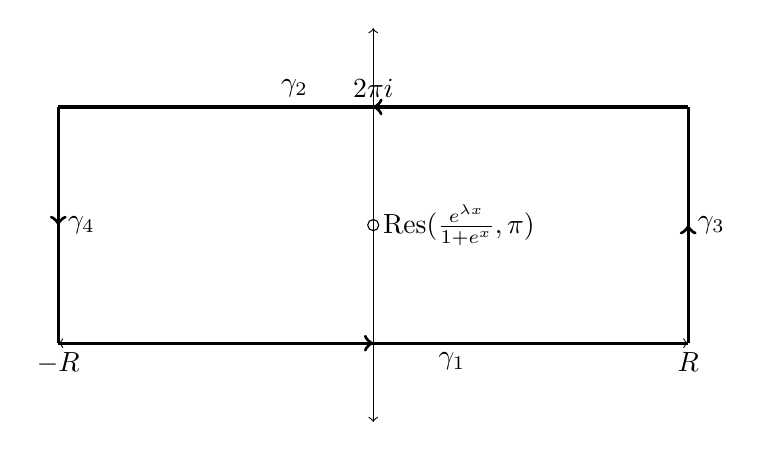
\begin{tikzpicture}
                                                                        \draw [<->] (-4, 0) -- (4, 0);
                                                                        \draw [<->] (0, -1) -- (0, 4);
                                                                        \node [below] at (-4, 0) {$-R$};
                                                                        \node [below] at (4, 0) {$R$};
                                                                        \node [below] at (1, 0) {$\gamma_1$};
                                                                        \node [above] at (-1, 3) {$\gamma_2$};
                                                                        \node [above] at (0, 3) {$2\pi i$};
                                                                        \node [right] at (4, 1.5) {$\gamma_3$};
                                                                        \node [right] at (-4, 1.5) {$\gamma_4$};
                                                                        \draw (0,1.5) circle[radius=2pt];
                                                                        \node [right] at (0, 1.5) {$\Res( \frac{e^{\lambda x}}{1 + e^x}, \pi)$};
                                                                        \begin{scope}[very thick,decoration={
                                                                            markings,
                                                                                mark=at position 0.5 with {\arrow{>}}}
                                                                                    ] 
                                                                                    \draw[postaction={decorate}] (-4,0) -- (4,0);
                                                                                    \draw[postaction={decorate}] (4,0) -- (4,3);
                                                                                    \draw[postaction={decorate}] (4,3) -- (-4,3);
                                                                                    \draw[postaction={decorate}] (-4,3) -- (-4,0);
                                                                                    \end{scope}
                                                                                    \end{tikzpicture}
                                                                                    }
                                                                                    \begin{align*}
                                                                                    \int_{\gamma_1}dz +\int_{\gamma_2}dz &= \int_{\gamma_1}dz -\int_{-\gamma_2}dz\\
                                                                                    &= \int_{-R}^R \frac{e^{\lambda x}}{1+e^x} - \frac{e^{\lambda (x+2\pi i)}}{1+e^{x+2\pi i}} dx\\
                                                                                    &= \int_{-R}^R \frac{e^{\lambda x} - e^{\lambda x +\lambda2\pi i}}{1+e^x}dx\\
                                                                                    &= (1 -e^{\lambda2\pi i})\int_{-R}^R \frac{e^{\lambda x}}{1+e^x}dx\\
                                                                                    &= (1 -e^{\lambda2\pi i})\int_{\gamma_1}dz 
                                                                                    \end{align*}
                                                                                    \begin{align*}
                                                                                    \abs{\int_{\gamma_3}dz} &= \abs{\int_0^{2\pi i} \frac{ie^{\lambda R + \lambda ti}dt}{1 + e^{R+ti}}}\\
                                                                                    &= \abs{\int_0^{2\pi} \frac{e^{\lambda R + \lambda ti} dt}{1 + e^{R+ti}}}\\
                                                                                    &\leq \abs{\int_0^{2\pi} \frac{e^{\lambda R} dt}{e^{R}}} = 2\pi e^{R(\lambda - 1)} \underset{R\to\infty}{\to} 0
                                                                                    \end{align*}
                                                                                    \begin{align*}
                                                                                    \abs{\int_{\gamma_4}dz} &= \abs{\int_0^{2\pi} \frac{-ie^{-\lambda R + \lambda ti}dt}{1 + e^{-R+ti}}}\\
                                                                                    &\leq 2\pi \sup \abs{\frac{e^{\lambda R+\lambda ti}}{1 + e^{R+ti}}}\\
                                                                                    &\leq 2\pi \abs{\frac{e^{\lambda R}}{1 + e^{R}}} \underset{R\to -\infty}{\to} \frac{0}{1} = 0
                                                                                    \end{align*}
                                                                                    Now by the residue theorem, 
                                                                                    \[
                                                                                    (1-e^{\lambda 2\pi i})\int_{\gamma_1}dz= \int_{\gamma_1+\gamma_2+\gamma_3+\gamma_4} dz  =  2\pi i \Res(\frac{e^{\lambda x}}{1+e^x}, i\pi)
                                                                                    \]

                                                                                    We can compute the residue at the simple pole 
                                                                                    \[
                                                                                     \Res(\frac{e^{\lambda x}}{1+e^x}, i\pi) = \lim_{x\to i\pi} \frac{e^{\lambda x}(x-i\pi)}{1-e^x}\big|_{x=i\pi} = \frac{\lambda e^{\lambda x}(x-i\pi) + e^{\lambda x}}{-e^x}|_{x=i\pi} = e^{i\pi\lambda}
                                                                                     \]

                                                                                     And now we can use the last two formulas to solve for the desired integral:
                                                                                     \[
                                                                                     \int_{\gamma_1}dz = \frac{2\pi i e^{i\pi \lambda}}{1 - e^{2\pi i \lambda}}
                                                                                     \]
                                                                                     \end{solution}
                                                                                     \begin{problem}
                                                                                       Evaluate the integral $\displaystyle\int_{0}^{2\pi} \frac{1}{3 + \sin^2 x} \, dx$.
                                                                                       \end{problem}
                                                                                       \begin{solution}
                                                                                       Rewrite $\sin x$ as follows:
                                                                                       \[
                                                                                       \sin x = \frac{e^{ix} - \frac{1}{e^{ix}}}{2i}
                                                                                       \]

                                                                                       Now let $\gamma=e^{ix}$ be the positively oriented unit circle.
                                                                                       \begin{align*}
                                                                                       \int_{0}^{2\pi} \frac{dx}{3 + \sin^2 x} \, dx &= 
                                                                                       \int_{0}^{2\pi} \frac{dx}{3 + \left(\frac{e^{ix} - \frac{1}{e^{ix}}}{2i}\right)^2}\\
                                                                                       &= \int_{0}^{2\pi} \frac{ie^{ix}dx}{ie^{ix}\left(3 - \left(\frac{e^{ix} - \frac{1}{e^{ix}}}{2}\right)^2\right)}\\
                                                                                       &= \int_\gamma \frac{dz}{iz\left(3 - \left(\frac{z - \frac{1}{z}}{2}\right)^2\right)}
                                                                                       \end{align*}

                                                                                       We can now try to apply the residue theorem. We need to find poles of the function 
                                                                                       $f(z) = \frac{-i}{z(3 - (\frac{z - \frac{1}{z}}{2})^2)}$ in the unit circle.
                                                                                       $z=0$ is a removable discontinuity since the second factor grows as fast as $\frac{1}{z^2}$ there, so the only poles are roots of the second factor. We can solve it with the quadratic formula and expand
                                                                                       \begin{align*}
                                                                                       3 - (\frac{z - \frac{1}{z}}{2})^2 &= 
                                                                                       \frac{4}{z^2}\left(3z^2 - (\frac{z^2 - 1}{2})^2\right)\\
                                                                                       &= \frac{4}{z^2}\left(  (z-(2-\sqrt{3}))(z-(2+\sqrt{3}))(z-(-2-\sqrt{3}))(z-(-2+\sqrt{3}))\right)
                                                                                       \end{align*}

                                                                                       The roots in the unit circle can be found with the quadratic formula as $\pm (2-\sqrt{3})$.
                                                                                       \begin{align*}
                                                                                       \Res(f, 2-\sqrt{3}) &= 
                                                                                       \frac{-4iz}{(z-(-2+\sqrt{3}))(z-(2+\sqrt{3}))(z-(-2-\sqrt{3}))}\big|_{z=2-\sqrt{3}}\\
                                                                                       &= \frac{-4iz}{2z\cdot 4\cdot 2\sqrt{3}} = \frac{-i}{4\sqrt{3}}
                                                                                       \end{align*}
                                                                                       \begin{align*}
                                                                                       \Res(f, 2+\sqrt{3}) &= 
                                                                                       \frac{-4iz}{(z-(2-\sqrt{3}))(z-(2+\sqrt{3}))(z-(-2-\sqrt{3}))}\big|_{z=-2+\sqrt{3}}\\
                                                                                       &= \frac{-4iz}{2z\cdot 4\cdot 2\sqrt{3}} = \frac{-i}{4\sqrt{3}}
                                                                                       \end{align*}
                                                                                       Now we can finally apply the residue formula to obtain the value of the desired integral:
                                                                                       \begin{align*}
                                                                                       2\pi i 
                                                                                       \left(\frac{-i}{4\sqrt{3}}+ \frac{-i}{4\sqrt{3}}\right) = \frac{\pi}{\sqrt{3}}
                                                                                       \end{align*}

                                                                                       \end{solution}
                                                                                       \begin{problem}
                                                                                         Evaluate the integral $\displaystyle \int_0^\pi \log \sin x \, dx$.
                                                                                         \end{problem}
                                                                                         \begin{solution}
                                                                                         \begin{align*}
                                                                                         \int_0^\pi \log \sin x dx &= \int_0^\pi \log \abs{\frac{e^{ix} - e^{-ix}}{2i}} dx\\
                                                                                         &= \int_0^\pi \log \abs{\frac{(e^{ix})(e^{ix} - e^{-ix})}{i}} dx - \int_0^\pi \log 2 dx \\
                                                                                         &= \int_0^\pi \log \abs{1 - e^{2ix}} dx - \pi \log 2
                                                                                         \int_0^\pi \log \sin x dx &= \frac{1}{2}\lim_{r^- \to 1}\int_0^{2\pi} \log \abs{1 - re^{ix}} dx - \pi \log 2\\
                                                                                         \end{align*}
                                                                                         Now we use the fact that for functions $f$ holomorphic on a disk of radius $r$ about the point $z_0$, 
                                                                                         \[
                                                                                         f(z_0) = \frac{1}{2\pi}\int_0^{2\pi} f(z_0+re^{i\theta})d\theta
                                                                                         \]
                                                                                         Applying this to $z_0=1, f=\log$:
                                                                                         \begin{align*}
                                                                                         \lim_{r^- \to 1}\int_0^{2\pi} \log (1 - e^{ix}) dx &= \lim_{r^-\to 1} \log 1 = 0
                                                                                         \end{align*}
                                                                                         And we conclude that
                                                                                         \[
                                                                                         \int_0^\pi \log \sin x \, dx = -\pi\log 2
                                                                                         \]
                                                                                         \end{solution}
                                                                                         \begin{problem}
                                                                                           Evaluate the integral $\displaystyle\int_{-\infty}^{\infty} \frac{1-x}{1-x^7} \, dx$.
                                                                                           \end{problem}
                                                                                           \begin{solution}
                                                                                           Let $f = \frac{1-x}{1-x^7} = \frac{1}{1+x+x^2+x^3+x^4+x^5+x^6}$ and $\zeta$ be the 7th root of unity with the smallest counterclockwise nonzero angle to the positive x axis.
                                                                                           We will compute the integral on the half circle contour as $R\to\infty$.

                                                                                           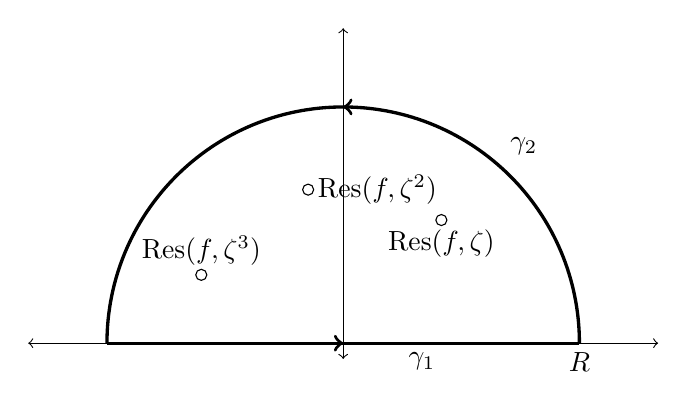
\begin{tikzpicture}
                                                                                           \draw [<->] (-4, 0) -- (4, 0);
                                                                                           \draw [<->] (0, -.2) -- (0, 4);
                                                                                           \node [below] at (3, 0) {$R$};
                                                                                           \node [below] at (1, 0) {$\gamma_1$};
                                                                                           \node [right] at (2, 2.5) {$\gamma_2$};
                                                                                           \draw (1.247, 1.564) circle[radius=2pt];
                                                                                           \draw (-.445, 1.95) circle[radius=2pt];
                                                                                           \draw (-1.802, 0.868) circle[radius=2pt];
                                                                                           \node [below] at (1.247, 1.564) {$\Res(f, \zeta)$};
                                                                                           \node [right] at (-.445, 1.95) {$\Res(f, \zeta^2)$};
                                                                                           \node [above] at (-1.802, 0.868) {$\Res(f, \zeta^3)$};
                                                                                           \begin{scope}[very thick,decoration={
                                                                                               markings,
                                                                                                   mark=at position 0.5 with {\arrow{>}}}
                                                                                                       ] 
                                                                                                       \draw[postaction={decorate}] (-3,0) -- (3,0);
                                                                                                       \draw[postaction={decorate}] (3, 0) arc [radius=3, start angle=0, end angle=180];
                                                                                                       \end{scope}
                                                                                                       \end{tikzpicture}

                                                                                                       The value of the integral on the outer curve $\gamma_2$ is 0:
                                                                                                       \[
                                                                                                       \int_{\gamma_2} \frac{1-z}{1-z^7} \leq \pi R \sup_{|z|=R} \frac{\abs{1-z}}{\abs{1-z^7}} \in O(R^{-6}) 
                                                                                                       \]
                                                                                                       Using the residue theorem, we can get the value of the integral by multiplying the residues by $2\pi i$. Unfortunately the residues are nasty to compute, so we will have a nasty expression.

                                                                                                       \begin{align*}
                                                                                                           \Res(f, \zeta^p) = \lim_{z\to \zeta^p} \frac{z-\zeta^p}{\prod_{k=1}^6 (z-\zeta^k)} = \frac{1}{\prod_{1\leq k \leq 6, k\neq p}^5 (\zeta^p-\zeta^k)}
                                                                                                           \end{align*}
                                                                                                           It's easy enough to numerically compute that none of these terms are 0, and consequentally that the computation is indeed valid.
                                                                                                           \begin{code}
                                                                                                           import cmath # using python
                                                                                                           zeta = complex(0.6234898018587336, 0.7818314824680298)
                                                                                                           res = [1/reduce(operator.mul, [pow(zeta, p) - pow(zeta,k) for k in range(1, 7) if k != p], 1) for p in range(1, 4)]
                                                                                                           >> [(-0.12085867654500679+0.02758520424482756j), (-0.09692113342087182-0.2012588073284831j), (0.21777980996587906-0.173673603083655j)]
                                                                                                           \end{code}
                                                                                                           And then we can get the answer by summing the residues and multiplying.
                                                                                                           \[
                                                                                                           \lim_{R\to \infty} \int_{\gamma_1} fdz = \int_{-\infty}^{\infty} f dz = 2\pi i \sum_{p=1}^3{\Res(f, \zeta^p)}
                                                                                                           \]
                                                                                                           \begin{code}
                                                                                                           sum(res)*2*cmath.pi * complex(0, 1)
                                                                                                           >> (2.182446862280324+2.964688223307337e-15j)
                                                                                                           \end{code}
                                                                                                           It's about 2.18.
                                                                                                           \end{solution}
                                                                                                           \begin{problem}
                                                                                                             Show that $f(z) = z^5 + 15z - 1$ has five zeros in $B_2(0)$, and one zero in $B_{1/15}(0)$.
                                                                                                             \end{problem}
                                                                                                             \begin{solution}
                                                                                                             First we will show that on $B_2(0)$, $\abs{z^5} > \abs{15z-1}$. By the triangle inequality, $\abs{15z-1} \leq \abs{15z} + \abs{1} = 31$, and $\abs{z^5} = 2^5 = 32$.

                                                                                                             Now we can apply Rouch\'e's theorem to say that $z^5$ and $z^5+15z-1$ have the same number of zeros in the ball of radius 2 counted with multiplicity, so $f(z)$ must have $5$ zeros in the ball.

                                                                                                             Next consider the ball of radius $\frac{1}{15}$. The function $15z-(1-10^{-9})$ has exactly one zero in this ball; we hope to apply Rouch\'e's theorem again by showing that 
                                                                                                             \[
                                                                                                             \abs{15z-1+10^{-9}} \geq \abs{z^5 - 10^{-9}}
                                                                                                             \]
                                                                                                             We can just apply the triangle inequality again:
                                                                                                             \[
                                                                                                             \abs{15z-1+10^{-9}} \geq 14 + 10^{-9} \geq \frac{1}{15}^5 - 10^{-9} \geq \abs{z^5 - 10^{-9}}
                                                                                                             \]
                                                                                                             Then we can confirm that there is one zero in the ball of radius $\frac{1}{15}$.

                                                                                                             \end{solution}
                                                                                                             \begin{problem}\label{form-at-infinity}
                                                                                                             Set $w = 1/z$ and compute $f(w) \, dw$ in terms of $f(z) \, dz$.
                                                                                                             \end{problem}
                                                                                                             \begin{solution}
                                                                                                             If $w=\frac{1}{z}$, differentiating both sides we get that $dw = \frac{-dz}{z^2}$. Thus $f(w) dw = -f(\frac{1}{z})\frac{dz}{z^2}$

                                                                                                             \end{solution}
                                                                                                             \section{Exploration}

                                                                                                             \begin{problem}
                                                                                                               Fix $w \in \R$ with $w>0$.  By the intermediate value theorem, the
                                                                                                                 polynomial $f(z) = z^4 + 4w^3 z - 1$ has a real root in the interval
                                                                                                                   $(-\infty,0)$ and another in $(0,1)$, along with two complex roots
                                                                                                                     $a \pm bi$.  Use Gauss-Lucas (\ref{gauss-lucas}) and Rouch\'e's
                                                                                                                       (\ref{rouches-theorem}) theorem to describe a subset of $\C$
                                                                                                                         containing $a\pm bi$.
                                                                                                                         \end{problem}
                                                                                                                         \begin{solution}

                                                                                                                         We can use Rouch\'e's theorem to show that the roots lie in the ball of radius $\max(2w, \sqrt{2})$. Under these conditions we can prove the inequality $|z^4|>|4w^3z - 1|$, and since $z^4$ has 4 zeros in the ball, so must $f$.

                                                                                                                         To prove the inequality: Suppose that $w>\sqrt[4]{1/8}$. Then 
                                                                                                                         \begin{align*}
                                                                                                                         &8w^4 > 1 \\
                                                                                                                         \implies &16w^4 > 8w^3 + 1\\
                                                                                                                         \implies &\abs{z^4} > \abs{4zw^3 - 1} \quad \text{ if } \abs{z} = 2w
                                                                                                                         \end{align*}
                                                                                                                         Otherwise, we must have that 
                                                                                                                         \[w<\sqrt[4]{1/8}< \sqrt[3]{\frac{3}{4\sqrt{2}}}\]
                                                                                                                         which implies that
                                                                                                                         \begin{align*}
                                                                                                                         3 > 4\sqrt{2}w^3\\
                                                                                                                         &\implies 4 > 4\sqrt{2}w^3 - 1\\
                                                                                                                         &\implies \abs{z^4} > \abs{4zw^3 - 1} \quad \text{ if } \abs{z} = \sqrt{2}
                                                                                                                         \end{align*}
                                                                                                                         In either case, the inequality is satisfied.

                                                                                                                         By Gauss-Lucas, the roots of $f$ contain the convex hull of the roots of $f'(z) = 4z^3+4w^3$, which are cubic roots of $w$. WLOG let $b\geq 0$. This implies that $b > \frac{\sqrt{3}w}{2}$. Combining this with the fact that $a+bi$ is contained in the ball of radius $\max(2w, \sqrt{2})$, we get a somewhat restricted set of locations for the roots.

                                                                                                                         We can restrict it a bit more if needed by considering the convex hull further: Let $\zeta_1 = w(\frac{\sqrt{3}}{2}+\frac{i}{2})$. Since the real roots are all on the line from $-\max(2w, \sqrt{2})$ to $1$, $a+bi$ is above the line from 1 to $\zeta_1$ and the line from $-\max(2w, \sqrt{2})$ to $\zeta_1$. And if $w>1$, then the real part of the roots is greater than $w.$ 
                                                                                                                         \end{solution}
                                                                                                                         \begin{problem}
                                                                                                                           What is the correct definition of $\Res(f,\infty)$?  Generally, we
                                                                                                                             would shift the viewport by replacing $f$ with the function
                                                                                                                               $g(z) = f(1/z)$ and then we study $g$ near $z = 0$ in order to
                                                                                                                                 investigate ``$f$ near $\infty$.''  Does \ref{form-at-infinity} help
                                                                                                                                   here?
                                                                                                                                   \end{problem}
                                                                                                                                   \begin{solution}
                                                                                                                                   Le $\gamma_R$ be the circle of radius $R$ centered at 0.
                                                                                                                                   The residue of $f$ at $\infty$ is kinda given by the formula
                                                                                                                                   \[
                                                                                                                                   \lim_{R \to \infty k} \int_{\gamma_R} \frac{f(w)dw}{w}
                                                                                                                                   \]
                                                                                                                                   Except that the part of the circle that is inside is backwards.

                                                                                                                                   We fix this by inverting everything using the subsitution $w=\frac{1}{z}$ investigated in $\ref{form-at-infinity}$ to get the formula
                                                                                                                                   \[
                                                                                                                                   \lim_{R^+\to 0} \int_{\gamma_R} -zg(z)\frac{dz}{z^2} = \lim_{R^+\to 0} \int_{\gamma_R} -g(z)\frac{dz}{z} 
                                                                                                                                   \]
                                                                                                                                   Except that since we inverted everything, we are now travelling on $\gamma$ in the clockwise direction. To fix this we get rid of the negative sign, and see that we are looking for the coefficent of $\frac{1}{z}$ in the taylor series of $g(z)$, which is nothing but the coefficient of $z$ in the taylor series of $f(z)$.
                                                                                                                                   \end{solution}
                                                                                                                                   \begin{problem}\label{rouches-theorem}Suppose $U$ is an open set containing the closed disk $D_r(z_0)$ and
                                                                                                                                     $f, g : U \to \C$ are holomorphic functions satisfying
                                                                                                                                       \[
                                                                                                                                           \abs{f(z)} > \abs{g(z)}
                                                                                                                                             \]
                                                                                                                                               for $z \in \partial D_r(z_0)$.  Prove \textbf{Rouch\'e's theorem}
                                                                                                                                                 that $f$ and $f+g$ have the same number of zeros, counted with
                                                                                                                                                   multiplicity, in $B_r(z_0)$.  (This is sometimes called the dog
                                                                                                                                                     leash theorem---can you see why?)
                                                                                                                                                     \end{problem}
                                                                                                                                                     \begin{solution}
                                                                                                                                                     The argument principal tells us that for any holomorphic function $f$, the number of roots of $f$ inside of a positively oriented jordan curve $\gamma$ is given by
                                                                                                                                                      $\frac{1}{2\pi i}\int_\gamma \frac{f'}{f} dz.$

                                                                                                                                                      In particular, the number of zeros of $f+g = f(1 + \frac{g}{f})$ is
                                                                                                                                                      \begin{align*}
                                                                                                                                                      \frac{1}{2\pi i}\int_\gamma \frac{(f(1 + \frac{g}{f}))'}{f(1 + \frac{g}{f})}dx &=
                                                                                                                                                      \frac{1}{2\pi i}\int_\gamma \frac{f'}{f} + \frac{(1+\frac{g}{f})'}{1 + \frac{g}{f}}dx 
                                                                                                                                                      \end{align*}
                                                                                                                                                      Thus it suffices to show that the term 
                                                                                                                                                      \(
                                                                                                                                                      \int_\gamma \frac{(1+\frac{g}{f})'}{1 + \frac{g}{f}}dx
                                                                                                                                                      \)
                                                                                                                                                      vanishes. Since $1+\frac{g}{f}>0$ on the boundary of $D_r(z_0)$, the function is analytic on the boundary, and since $\abs{f}>\abs{g}$, the function $1+\frac{g}{f}$ is analytic and always positive, so it has no zeros. By the argument principal, the term must evaluate to 0.
                                                                                                                                                      \end{solution}
                                                                                                                                                      \begin{problem}
                                                                                                                                                        Use \ref{rouches-theorem} to give another proof of the Fundamental Theorem of Algebra.
                                                                                                                                                        \end{problem}
                                                                                                                                                        \begin{solution}
                                                                                                                                                        Let $p(x) = \sum_{k=1}^d a_kx^k$ be a degree $d$ polynomial with $a_d\neq 0$. Then we can choose a circle $B_r(0)$ of sufficently big radius so that the leading term dominates on $\partial B_r(0)$:
                                                                                                                                                        \[
                                                                                                                                                        \abs{a_dx^d} \geq \abs{\sum_{k=1}^d a_kx^k}
                                                                                                                                                        \]
                                                                                                                                                        We should also ensure that $r > \sqrt[d]{a_d}$, to observe that $a_dx^d$ has exactly $d$ roots in the circle corresponding to the scaled $d$th roots of unity. By Rouch\'e's theorem, this means that $p(x)$ also has exactly $d$ roots in this big circle. And, in fact, in any circle of even larger size, so we can even say that $p(x)$ has exactly $d$ roots in $\C$.
                                                                                                                                                        \end{solution}
                                                                                                                                                        \begin{problem}
                                                                                                                                                          It is important to recognize patterns in how residues equip us to evaluate integrals, so that, when presented with a fresh integration problem, we have some ideas about the best tool for the task.  Develop a tool for evaluating
                                                                                                                                                            \[
                                                                                                                                                                \int_0^{2\pi} f(\cos \theta,\sin \theta) \, d\theta
                                                                                                                                                                  \]
                                                                                                                                                                    via residues.  Here $f$ is a rational function, explain how to make
                                                                                                                                                                      the substitution $z = e^{i\theta}$ to rewrite
                                                                                                                                                                        $f(\cos \theta,\sin \theta)$ in terms of $z$, and
                                                                                                                                                                          similarly rewrite $d\theta$ in terms of
                                                                                                                                                                            $dz$ to reduce the given integral to a certain contour integral.
                                                                                                                                                                            \end{problem}
                                                                                                                                                                            \begin{solution}
                                                                                                                                                                            Let $z=e^{i\theta}$ so that $dz = ie^{i\theta} d\theta$. Then $d\theta = \frac{dz}{iz}$ and 
                                                                                                                                                                            \begin{gather*}
                                                                                                                                                                            \cos\theta = \frac{e^{i\theta} + e^{-i\theta}}{2} = \frac{z+z^{-1}}{2}\\
                                                                                                                                                                            \sin\theta = \frac{e^{i\theta} - e^{-i\theta}}{2i} = \frac{z-z^{-1}}{2i}
                                                                                                                                                                            \end{gather*}
                                                                                                                                                                            So the integral becomes
                                                                                                                                                                            \[
                                                                                                                                                                            \int_\gamma f(\frac{z+z^{-1}}{2},\frac{z-z^{-1}}{2i})\frac{dz}{iz}
                                                                                                                                                                            \]
                                                                                                                                                                            Where $\gamma$ is the image of $e^{i\theta}$ for $0\leq \theta \leq 2\pi$, that is, the positively oriented unit circle 
                                                                                                                                                                            \[\gamma:[0, 2\pi] \to \C\qquad \gamma(\theta)= e^{i\theta}.\]

                                                                                                                                                                            Since $f$ is a rational function, we have a rational function in $z$ so it is meromorphic with finitely many poles $\{z_k\}_{k=1}^n$ in the unit circle and the residue theorem can be used to evaluate the integrals:
                                                                                                                                                                            \[
                                                                                                                                                                                \int_0^{2\pi} f(\cos \theta, \sin\theta) d\theta =  2\pi i \sum_{k=1}^n \Res(f(\frac{z+z^{-1}}{2},\frac{z-z^{-1}}{2i}\frac{1}{iz} ), z_k)
                                                                                                                                                                                \]
                                                                                                                                                                                \end{solution}
                                                                                                                                                                                \begin{problem}\label{summation-theorem}Sometimes the residue calculus
                                                                                                                                                                                  permits us to sum series.

                                                                                                                                                                                    Suppose $f$ is meromorphic with poles $z_1,\ldots,z_N$ with $z_j \not\in \Z$.  Our goal is a formula
                                                                                                                                                                                      \[
                                                                                                                                                                                          \sum_{n=-\infty}^{\infty} f(n) = - \sum_{j=1}^N \Res(g, z_j)
                                                                                                                                                                                            \]
                                                                                                                                                                                              where $g(z) = \pi \cot(\pi z) f(z)$.  \textit{Hint:} Consider a square contour $R$ centered at the origin with side-length $2N+1$.  You may assume that $\pi \cot(\pi z)$ is bounded on $R$ independent of $N$.  You will then need to impose some bound on $f$ on the contour $R$.
                                                                                                                                                                                              \end{problem}
                                                                                                                                                                                              \begin{solution}
                                                                                                                                                                                              Let's compute the contour integral $I=\int_R g(z)dz$ in two different ways. First, using the residue theorem, we have that 
                                                                                                                                                                                              \begin{equation}\label{Residue_eq_q}
                                                                                                                                                                                              \frac{I}{2\pi i} = \sum_{j=1}^N \Res(g,z_i) + \sum_{k=-\infty} ^\infty \Res(g, k).
                                                                                                                                                                                              \end{equation}
                                                                                                                                                                                              We can compute the residue of $g$ at $k$
                                                                                                                                                                                              \[
                                                                                                                                                                                              \Res(\pi\cot(\pi z)f(z), k) = \lim_{z\to k} \pi\cos(\pi z)f(z)\frac{(z-k)}{\sin(\pi z)} = \lim_{z\to k} \pi\cos(\pi z)f(z)\frac{(z-k)}{\sin(\pi z)} 
                                                                                                                                                                                              \]

                                                                                                                                                                                              Thus if we can show that $I=0$, we get the desired equality  from \eqref{Residue_eq_q}.
                                                                                                                                                                                              \[
                                                                                                                                                                                              0 = \sum_{j=1}^N \Res(g,z_i) + \sum_{k=-\infty} ^\infty f(k).
                                                                                                                                                                                              \]

                                                                                                                                                                                              Second, let's compute $\int_R g(z)dz$ directly, aiming for it to be 0.
                                                                                                                                                                                              \[
                                                                                                                                                                                              \lim_{N\to\infty} \int_R g(z) dz \leq (4(2N+1))\sup_{z\in R}(g(z))
                                                                                                                                                                                              \]
                                                                                                                                                                                              Since $\pi\cot(\pi z)$ is bounded, it suffices for the growth rate of $f(z)$ to be asymptotically slowed than that of $8N+4$: $f(|z|) \in \omega(|z|)$.

                                                                                                                                                                                              If so, we can conclude that $I=0$, proving the claim.
                                                                                                                                                                                              \end{solution}
                                                                                                                                                                                              \begin{problem}
                                                                                                                                                                                                Apply \ref{residue-coth} and \ref{summation-theorem} to evaluate
                                                                                                                                                                                                  \[
                                                                                                                                                                                                      \sum_{n=-\infty}^\infty \frac{1}{n^2 + b^2}.
                                                                                                                                                                                                        \]
                                                                                                                                                                                                        \end{problem}
                                                                                                                                                                                                        \begin{solution}
                                                                                                                                                                                                        Let $f(n) = \frac{1}{n^2+b^2}$. We assume $bi \not \in \Z$ so that the sum is finite. Then in the previous problem, $g(n) = \frac{\pi\cot(\pi z)}{z^2 + b^2}$. By \ref{residue-coth}, the residue at $\pm bi$ is $\frac{\pi\cot(\pm \pi bi)}{\pm 2bi}$, so the sum of the residues is $-\frac{\pi \coth{\pi b}}{b}$ and thus the sum is $\frac{\pi \coth{\pi b}}{b}$.
                                                                                                                                                                                                        \end{solution}
                                                                                                                                                                                                        \section{Prove or Disprove and Salvage if Possible}

                                                                                                                                                                                                        \begin{problem}\label{zero-residue-not-enough}Suppose $f : D_r(z_0) \to \C$ is holomorphic.  The residue
                                                                                                                                                                                                          $\Res(f,z_0)$ vanishes if and only if the singularity $z_0$ is
                                                                                                                                                                                                            removable.
                                                                                                                                                                                                            \end{problem}
                                                                                                                                                                                                            \begin{solution}
                                                                                                                                                                                                            This is true for stupid reasons: if $f$ is holomorphic on a disk surrounding $z_0$, then $f$ has no singularity at $z_0$, so if a singularity exists, it is surely removable. If it is merely meromorphic, a counterexample like $\frac{1}{z^2}$ suffices, since it has residue $0$ but no removable singularity at $0$.

                                                                                                                                                                                                            However, if the singularity is removable, the residue will vanish, since after removing the singularity, $f$ is holomorphic on a small ball containing $z_0$, so the residue must vanish.


                                                                                                                                                                                                            \end{solution}
                                                                                                                                                                                                            \begin{problem}\label{open-mapping-theorem}If $U \subset \C$ is open
                                                                                                                                                                                                              and $f : U \to \C$ is holomorphic, then $f(U)$ is
                                                                                                                                                                                                                open. % missing nonconstant, can be proved from rouche
                                                                                                                                                                                                                \end{problem}
                                                                                                                                                                                                                \begin{solution}
                                                                                                                                                                                                                No, consider $f(z)=0$. If we don't allow $f$ to be a constant, then it is true.

                                                                                                                                                                                                                Choose some arbitrary point $z_0\in U$ with $f(z_0)=w_0$. Now consider a series of open balls $\{B_{1/n}(z_0)\}_{n\in\N}$. We can surely find an $n$ where the $n$th ball is contained in $U$ since $U$ is open. Furthermore, by the identity theorem, there is an $n$ where the $n$th ball does not contain any point $z_1$ with $f(z_1)=w_0$ - otherwise, we would have an infinite series of points $\{z_i\}$ containing their limit point where $f(z_i)=w$, implying by the identity theorem that $\forall z\in U, f(z) = w$. Call the first $n$ satsifying both conditions $N$.

                                                                                                                                                                                                                Let $\delta = (\inf_{z\in B_{1/N}(z_0)}\abs{f(z)-w_0})/2$, so that for all $z$ in this ball,
                                                                                                                                                                                                                \[
                                                                                                                                                                                                                \abs{f(z) - w_0 } \geq 2\delta.
                                                                                                                                                                                                                \]
                                                                                                                                                                                                                Choose some $w_1\in \partial D_\delta (f(z_0))$, so that 
                                                                                                                                                                                                                \[\delta \geq \abs{w_0-w_1}.
                                                                                                                                                                                                                \]

                                                                                                                                                                                                                To show that $f(U)$ is open, it suffices to show that any such $w_1$ is in the image of $f$, or equivalently that $f(z) - w_1$ has a zero. We know from the last paragraph that $f(z)-w_0$ has exactly one zero in $B_{1/N}(z_0)$, and that 
                                                                                                                                                                                                                \[
                                                                                                                                                                                                                \abs{f(z) - w_0} \geq \abs{w_0 - w_1}
                                                                                                                                                                                                                \]
                                                                                                                                                                                                                so by Rouche's theorem, $f(z)-w_0 +w_0-w_1 = f(z) - w_1$ has a zero in $B_{1/N}$. Thus $f(U)$ is open.
                                                                                                                                                                                                                \end{solution}


                                                                                                                                                                                                                \end{document}
